\chapter{Ανάλυση προτιμήσεων φοιτητών}
    \section{Υπάρχουσες έρευνες και σχετική βιβλιογραφία}
        Σε πολλές περιπτώσεις, η αποτελεσματικότητα των φοιτητών καθορίζεται κυρίως από την οργάνωσή τους και τον σωστό προγραμματισμό τους, τόσο στις ακαδημαϊκές όσο και στις προσωπικές τους υποχρεώσεις. Η σωστή διαχείριση χρόνου και προτεραιοτήτων είναι καθοριστική για την αποφυγή άγχους, την αύξηση της παραγωγικότητας και την επίτευξη των στόχων τους. Παρόλα αυτά, οι φοιτητές συχνά έρχονται αντιμέτωποι με προκλήσεις, όπως η αναβλητικότητα και η έλλειψη σωστής οργάνωσης για την ολοκλήρωση των καθημερινών τους καθηκόντων. Οι ερευνητικές προσπάθειες στον τομέα αυτό αναδεικνύουν τα εμπόδια που αντιμετωπίζουν οι φοιτητές και προσφέρουν πολύτιμες πληροφορίες για τη βελτίωση των δεξιοτήτων διαχείρισης εργασιών.

        \subsection{Προβλήματα διαχείρισης που αντιμετωπίζουν οι φοιτητές} \label{sec:student_problems}
            Σε έρευνα \cite{Fukuzawa2015} που διεξήχθη στο Πανεπιστήμιο του Τσουκούμπα της Ιαπωνίας, η οποία διερευνούσε τη διαχείριση του προγραμματισμού των εργασιών από την πλευρά των φοιτητών, παρατηρήθηκε πως η πλειοψηφία τους αντιμετωπίζει δυσκολίες στην εκκίνηση μιας νέας εργασίας. Οι βασικοί λόγοι που καταγράφηκαν περιλαμβάνουν: α) την έλλειψη χρόνου (26,9\%), β) την αγνόηση της εργασίας επειδή τη θεωρούσαν ελάσσονος σημασίας (15,7\%), γ) επειδή την ξέχασαν (12,3\%), δ) λόγω κακής συνεργασίας (11,2\%) και ε) επειδή ήταν κουραστική (8,9\%). Οι τρεις πρώτοι λόγοι, που καλύπτουν το μεγαλύτερο ποσοστό (54,9\%), αναφέρονται σε θέματα κακής οργάνωσης από την πλευρά των φοιτητών, υποδεικνύοντας την ανάγκη για αποτελεσματικότερα εργαλεία χρονοπρογραμματισμού.

            Παράλληλα, μια διαφορετική έρευνα \cite{Trujillo2020} καταδεικνύει πάλι πως το κυριότερο πρόβλημα που αντιμετωπίζουν οι φοιτητές είναι η σωστή δόμηση του προγράμματός τους. Παρατηρήθηκε ότι ο τρόπος με τον οποίο οργανώνουν το διάβασμά τους καθοδηγείται κυρίως από τις καταληκτικές ημερομηνίες των εργασιών τους, με αποτέλεσμα να παραμελούν άλλες σημαντικές ακαδημαϊκές δραστηριότητες, όπως η παρακολούθηση διαλέξεων. Αυτό οδηγεί σε ανισορροπία μεταξύ των ακαδημαϊκών τους υποχρεώσεων, επηρεάζοντας την απόδοσή τους συνολικά.

            Οι παραπάνω έρευνες οδήγησαν σε συγκεκριμένα συμπεράσματα. Πρώτον, η έλλειψη οργανωτικών δεξιοτήτων παραμένει ένας από τους κύριους παράγοντες που εμποδίζουν την αποτελεσματική διαχείριση των εργασιών από τους φοιτητές. Οι λόγοι αυτοί συνδέονται συχνά με την αναβλητικότητα και την έλλειψη εργαλείων που θα μπορούσαν να βοηθήσουν στην αποδοτικότερη οργάνωση των καθημερινών τους υποχρεώσεων. Δεύτερον, η ανάγκη για ένα δομημένο σύστημα προγραμματισμού είναι εμφανής, καθώς θα μπορούσε να παρέχει σαφείς προτεραιότητες και να συμβάλει στη μείωση του άγχους που προκαλείται από τις καταληκτικές ημερομηνίες. Συνεπώς, ένα αποτελεσματικό σύστημα διαχείρισης και προγραμματισμού των εργασιών, προσαρμοσμένο στις ανάγκες των φοιτητών, μπορεί να λειτουργήσει ως βασικό εργαλείο για την ενίσχυση της παραγωγικότητας και της επιτυχίας τους.

        \subsection{Χαρακτηριστικά που οι φοιτητές θα επιθυμούσαν σε μια εφαρμογή} \label{sec:student_preferences}
            Σε έρευνα \cite{Trujillo2020} που πραγματοποιήθηκε στο τμήμα Πληροφορικής του Πανεπιστημίου του Εδιμβούργου, αναδείχθηκαν κάποιες σημαντικές προτιμήσεις και απαιτήσεις της ακαδημαϊκής κοινότητας σχετικά με τη λειτουργικότητα των εφαρμογών διαχείρισης εργασιών. Η πλειοψηφία των συμμετεχόντων τόνισε τη σημασία της ύπαρξης ενός ενσωματωμένου ημερολογίου, το οποίο θα παρέχει τη δυνατότητα καταγραφής των ημερομηνιών έναρξης και λήξης για κάθε εργασία. Αυτή η λειτουργία θεωρήθηκε κρίσιμη για τη σωστή οργάνωση και τον προγραμματισμό των υποχρεώσεων, καθώς επιτρέπει στους χρήστες να έχουν σαφή εικόνα των προθεσμιών τους. Παράλληλα, υπογραμμίστηκε η αξία της χρωματικής ταξινόμησης (color-coding), η οποία διευκολύνει τη διάκριση μεταξύ διαφορετικών κατηγοριών ή τύπων εργασιών, ενισχύοντας τη διαφάνεια και την ευκολία χρήσης της εφαρμογής.

            Επιπλέον, οι συμμετέχοντες επισήμαναν την ανάγκη για ειδοποιήσεις/γνωστοποιήσεις, οι οποίες θα λειτουργούν ως υπενθυμίσεις για τις επερχόμενες προθεσμίες ή τις εκκρεμότητες που απαιτούν άμεση προσοχή. Εξίσου σημαντική θεωρήθηκε η ύπαρξη to-do λιστών, οι οποίες θα διαθέτουν λειτουργίες όπως ιεράρχηση των εργασιών, ομαδοποίηση σε κατηγορίες, και δυνατότητα εμφάνισης μπάρας προόδου. Αυτές οι δυνατότητες συμβάλλουν στην αποτελεσματικότερη παρακολούθηση της προόδου των εργασιών και στη δημιουργία μιας αίσθησης ολοκλήρωσης και επίτευξης στόχων.

            Ιδιαίτερο ενδιαφέρον παρουσίασε η πρόταση για την ενσωμάτωση ενός συστήματος ανταμοιβής, το οποίο στοχεύει στην ενθάρρυνση των φοιτητών να ολοκληρώνουν τις εργασίες τους εγκαίρως. Ένα τέτοιο σύστημα θα μπορούσε να περιλαμβάνει την εμφάνιση γραφικών στοιχείων όπως κομφετί ή εικονικά μετάλλια, ή την ανταμοιβή πόντων, συμβάλλοντας στη δημιουργία κινήτρων. Η εισαγωγή αυτού του συστήματος έχει σκοπό να ενισχύσει τη δέσμευση και την παραγωγικότητα των χρηστών, προσφέροντας έναν πιο διαδραστικό και ελκυστικό τρόπο διαχείρισης εργασιών. Με την ενσωμάτωση χαρακτηριστικών όπως τα προαναφερθέντα, τέτοιες εφαρμογές μπορούν να βελτιώσουν ουσιαστικά την παραγωγικότητα και την αποτελεσματικότητα, προσφέροντας παράλληλα μια ευχάριστη εμπειρία χρήσης.

    \section{Πρωτογενής έρευνα}
        Πέρα από τις υπάρχουσες έρευνες, στο πλαίσιο της διπλωματικής εργασίας πραγματοποιήθηκε νέα έρευνα με στόχο την κατανόηση των δυσκολιών που αντιμετωπίζουν οι φοιτητές στο καθημερινό προγραμματισμό των εργασιών τους, καθώς και την καταγραφή των χαρακτηριστικών που θεωρούν πιο χρήσιμα σε μια εφαρμογή διαχείρισης εργασιών. Η συλλογή αυτών των δεδομένων αποτέλεσε κρίσιμο βήμα για τη διαμόρφωση των απαιτήσεων της υπό ανάπτυξη εφαρμογής, διασφαλίζοντας ότι το τελικό προϊόν θα είναι όσο το δυνατόν πιο λειτουργικό και προσαρμοσμένο στις ανάγκες των φοιτητών.

        \subsection{Μεθοδολογία και δείγμα}
            Για τη συλλογή των δεδομένων, συγκεντρώθηκαν ποσοτικά στοιχεία μέσω ενός ερωτηματολογίου που δημιουργήθηκε στο Google Forms. Το ερωτηματολόγιο επικεντρωνόταν στους δύο βασικούς άξονες που αναλύθηκαν στις ενότητες \ref{sec:student_problems} και \ref{sec:student_preferences}.

            Η έρευνα πραγματοποιήθηκε σε ένα δείγμα 14 φοιτητών, γεγονός που διασφαλίζει τη συνάφεια των απαντήσεων τους με το αντικείμενο της έρευνας. Η συμμετοχή ήταν εθελοντική και οι φοιτητές απάντησαν στο ερωτηματολόγιο ανώνυμα. Η συλλογή των δεδομένων διήρκεσε μια εβδομάδα και ο σύνδεσμος για την πρόσβαση στο ερωτηματολόγιο διανεμήθηκε μέσω κοινωνικών δικτύων.

        \subsection{Ερωτηματολόγιο} \label{sec:pollstats}
            Τα ερωτήματα με τις πιθανές απαντήσεις που περιελάμβανε το ερωτηματολόγιο παρουσιάζονται παρακάτω:

            \begin{table}[H] \noindent\centering
                \caption{Ερωτηματολόγιο προτιμήσεων φοιτητών}
                \resizebox{0.7\textwidth}{!}{
                    \begin{tabular}{l|l}
                       \textbf{Ερωτήσεις} & \textbf{Πιθανές απαντήσεις}  \\
                        \midrule
                        Τι ηλικία έχεις; & 18-19 \\& 20-21 \\& 22-24 \\& 25+ \\
                        \midrule
                        Ποιο είναι το ακαδημαϊκό σου επίπεδο; & Προπτυχιακό \\& Μεταπτυχιακό \\& Διδακτορικό \\
                        \midrule
                        Τι σπουδάζεις; & (κείμενο σύντομης απάντησης) \\
                        \midrule
                        Σε ποιο έτος σπουδών είσαι; & 1ο, 2ο, 3ο, 4ο, 5ο, Επί πτυχίο \\
                    \end{tabular}}
                \label{tab:poll}
            \end{table}

            \begin{table}[H] \noindent\centering
                \resizebox{\textwidth}{!}{
                    \begin{tabular}{l|l}
                       \textbf{Ερωτήσεις} & \textbf{Πιθανές απαντήσεις}  \\
                        \midrule
                        Χρησιμοποιείς κάποιο εργαλείο για τη διαχείριση & Ναι \\
                        του χρόνου σου και των υποχρεώσεών σου; & Όχι, προγραμματίζω στο μυαλό μου \\
                        \midrule
                        Αν ναι, ποιο/α εργαλείο/α χρησιμοποιείς; & Εφαρμογές (π.χ., Ημερολόγιο, Notion, Todoist) \\& Υπενθυμίσεις στο κινητό ή υπολογιστή \\& Ημερολόγιο σε φυσική μορφή \\& Post-it ή άλλες χειρόγραφες σημειώσεις \\& Excel ή άλλα υπολογιστικά φύλλα \\& Άλλο \\
                        \midrule
                        Αν ναι, οι εργασίες που προγραμματίζεις & Υποχρεώσεις σχολής (π.χ., διάβασμα, εργασίες) \\
                        και οργανώνεις αφορούν περισσότερο... & Υποχρεώσεις καθημερινότητας (π.χ., ψώνια) \\
                        & Κοινωνικές δραστηριότητες (π.χ. χόμπι) \\& Προσωπική ανάπτυξη (π.χ., μαθήματα γλωσσών) \\& Προσωπική φροντίδα (π.χ., ραντεβού με γιατρούς) \\& Άλλο \\
                        \midrule
                        Αν ναι, σε κλίμακα από 1 έως 5, πόσο αποτελεσματικές & 1 -- 5 \\
                        θεωρείς τις μεθόδους διαχείρισης εργασιών που χρησιμοποιείς; & \\
                        \midrule
                        Τι δυσκολίες αντιμετωπίζεις & Αναβλητικότητα \\
                        στη διαχείριση των υποχρεώσεών σου; & Δυσκολία στην ιεράρχιση των εργασιών
                       \\& Πάρα πολλές υποχρεώσεις \\& Έλλειψη κινήτρων \\& Αδυναμία τήρησης προγράμματος \\& Απόσπαση προσοχής από social media \\& Έλλειψη χρόνου για σωστό προγραμματισμό \\& Αγωνία ή άγχος σχετικά με τις προθεσμίες \\& Κακή εκτίμηση του απαιτούμενου χρόνου \\
                        \midrule
                        Πόσο συχνά έχει τύχει να χάσεις κάποια προθεσμία (deadline); & Ποτέ, Σπάνια, Μερικές φορές, Συχνά, Πάντα \\
                        \midrule
                        Έχει τύχει να μην έχεις ξεκινήσει καν κάποια εργασία σου; & Ναι, Όχι \\
                        \midrule
                        Αν ναι, ποιοι ήταν οι λόγοι; & Έλλειψη χρόνου \\& Την ξέχασα \\& Κακή συνεργασία ομάδας \\& Ήταν κουραστική \\& Άλλο \\
                        \midrule
                        Πόσο συχνά αισθάνεσαι αγχωμένος/η από τον φόρτο των εργασιών σου; & Ποτέ, Σπάνια, Μερικές φορές, Συχνά, Πάντα \\
                        \midrule
                        Τι θεωρείς χρήσιμο σε μια εφαρμογή διαχείρισης εργασιών για φοιτητές; \\
                        \textit{Ύπαρξη ημερολογίου} & \textit{1 (καθόλου χρήσιμο) -- 5 (πολύ χρήσιμο)} \\
                        \textit{Ιεράρχιση εργασιών (χαμηλή, υψηλή προτεραιότητα)} & \textit{1 (καθόλου χρήσιμο) -- 5 (πολύ χρήσιμο)} \\
                        \textit{Κατηγοροποίηση εργασιών βάσει του χρώματός τους (color-coding)} & \textit{1 (καθόλου χρήσιμο) -- 5 (πολύ χρήσιμο)} \\
                        \textit{Ύπαρξη επαναλαμβανόμενων (recurring) εργασίες} & \textit{1 (καθόλου χρήσιμο) -- 5 (πολύ χρήσιμο)} \\
                        \textit{Σύστημα επιβράβευσης κατά την ολοκλήρωση μιας εργασίας} & \textit{1 (καθόλου χρήσιμο) -- 5 (πολύ χρήσιμο)} \\
                        \textit{Καλαίσθητο, φιλικό για τον χρήστη, γραφικό περιβάλλον} & \textit{1 (καθόλου χρήσιμο) -- 5 (πολύ χρήσιμο)} \\
                        \textit{Προειδοποίηση πριν λήξει η προθεσμία μιας εργασίας} & \textit{1 (καθόλου χρήσιμο) -- 5 (πολύ χρήσιμο)} \\
                        \midrule
                        Σε κλίμακα από 1 έως 5, πόσο πιθανό είναι να χρησιμοποιήσεις & 1 -- 5 \\
                        μια εφαρμογή σχεδιασμένη για τη διαχείριση εργασιών των φοιτητών;
                    \end{tabular}}
            \end{table}

        \subsection{Αποτελέσματα}
            Εν τέλει το δείγμα αποτελείται από 14 φοιτητές, με το 28.6\% (n = 4) να ανήκει στην ηλικιακή ομάδα 18--19 ετών, το 21.4\% (n = 3) στην ηλικιακή ομάδα 20--21 ετών, το 28.6\% (n = 4) στην ηλικιακή ομάδα 22--24 ετών και το 21.4\% (n = 3) στην ηλικιακή ομάδα 25+.

            Όσον αφορά το ακαδημαϊκό επίπεδο, το 71.4\% (n = 10) των συμμετεχόντων είναι προπτυχιακοί φοιτητές, ενώ το 14.3\% (n = 2) μεταπτυχιακοί και το 14.3\% (n = 2) διδακτορικοί φοιτητές.

            Σχετικά με το αντικείμενο σπουδών, 6 φοιτητές σπουδάζουν στο παρόν τμήμα, οι υπόλοιποι φοιτητές σπουδάζουν Επιστήμη Υλικών, Διοίκηση Επιχειρήσεων, Ιατρική, ΗΜΤΥ, Φιλολογία, και Διατροφολογία. Το 7.1\% (n = 1) των φοιτητών είναι στο 1ο έτος σπουδών, το 28.6\% (n = 4) στο 2ο έτος, το 21.4\% (n = 3) στο 3ο έτος, το 7.1\% (n = 1) στο 4ο έτος, το 14.3\% (n = 2) στο 5ο έτος, και το 21.4\% (n = 3) είναι επί πτυχίο.

            Σχετικά με τη χρήση εργαλείων για τη διαχείριση του χρόνου, το 64.3\% (n = 9) των φοιτητών χρησιμοποιούν κάποιο εργαλείο, ενώ το 35.7\% (n = 5) προγραμματίζουν τις υποχρεώσεις τους στο μυαλό τους. Από τους φοιτητές που χρησιμοποιούν εργαλεία, και οι 9 χρησιμοποιούν κάποια εφαρμογή, ενώ 2 από αυτούς επιπλέον χρησιμοποιούν υπενθυμίσεις ή ημερολόγιο σε φυσική μορφή.

            Όσον αφορά το είδος των εργασιών που προγραμματίζουν, και οι 9 φοιτητές αναφέρουν ότι προγραμματίζουν υποχρεώσεις σχολής και επίσης 4 από αυτούς προγραμματίζουν υποχρεώσεις καθημερινότητας, 3 κοινωνικές δραστηριότητες, 2 προσωπική ανάπτυξη και 3 προσωπική φροντίδα. Σε κλίμακα από 1 έως 5, 5 φοιτητές βαθμολογούν τις μεθόδους διαχείρισης εργασιών που χρησιμοποιούν με βαθμό 4, 4 φοιτητές με βαθμό 3, 3 φοιτητές με βαθμό 2 ενώ ένας φοιτητής με βαθμό 1.

            Σχετικά με τις δυσκολίες που αντιμετωπίζουν στη διαχείριση των υποχρεώσεών τους, 9 φοιτητές αναφέρουν ότι αντιμετωπίζουν απόσπαση προσοχής από social media, 6 φοιτητές αντιμετωπίζουν αναβλητικότητα, 5 φοιτητές αντιμετωπίζουν αγωνία ή άγχος σχετικά με τις προθεσμίες, 4 φοιτητές αντιμετωπίζουν αδυναμία τήρησης προγράμματος, 3 φοιτητές έχουν πάρα πολλές υποχρεώσεις ή έλλειψη κινήτρων, ενώ 2 φοιτητές έχουν δυσκολία στην ιεράρχηση των εργασιών τους, έλλειψη χρόνου για σωστό προγραμματισμό ή κακή εκτίμηση του απαιτούμενου χρόνου για τον προγραμματισμό τους.

            Σχετικά με τις προθεσμίες, το 42.9\% (n = 6) των φοιτητών αναφέρουν ότι μερικές φορές έχουν χάσει κάποια προθεσμία, το 21.4\% (n = 3) συχνά, το 14.3\% (n = 2) πάντα και ποτέ και το 7.1\% (n = 1) σπάνια. Όσον αφορά το αν έχει τύχει να μην έχουν ξεκινήσει κάποια εργασία τους, οι μισοί απάντησαν ότι ναι, ενώ οι υπόλοιποι όχι. Αν ναι, έχουν δοθεί 8 απαντήσεις (μια επιπλέον), με 2 απαντήσεις να αναφέρουν ότι η έλλειψη χρόνου ήταν ο λόγος που δεν ξεκίνησαν την εργασία τους, 2 απαντήσεις να αναφέρουν ότι την ξέχασαν, 2 απαντήσεις να αναφέρουν ότι ήταν κουραστική και μια απάντηση να αναφέρει πως ο λόγος ήταν η συνεργατικότητα που απαιτούσε η εργασία.

            Σχετικά με το αν αγχώνονται οι φοιτητές από τον φόρτο των εργασιών, το 42.9\% (n = 6) των φοιτητών αναφέρουν ότι συχνά αισθάνονται αγχωμένοι, το 28.6\% (n = 4) μερικές φορές, το 14.3\% (n = 2) σπάνια, το 7.1\% (n = 1) ποτέ και το 7.1\% (n = 1) πάντα.

            \begin{figure}[h!] \noindent \centering
                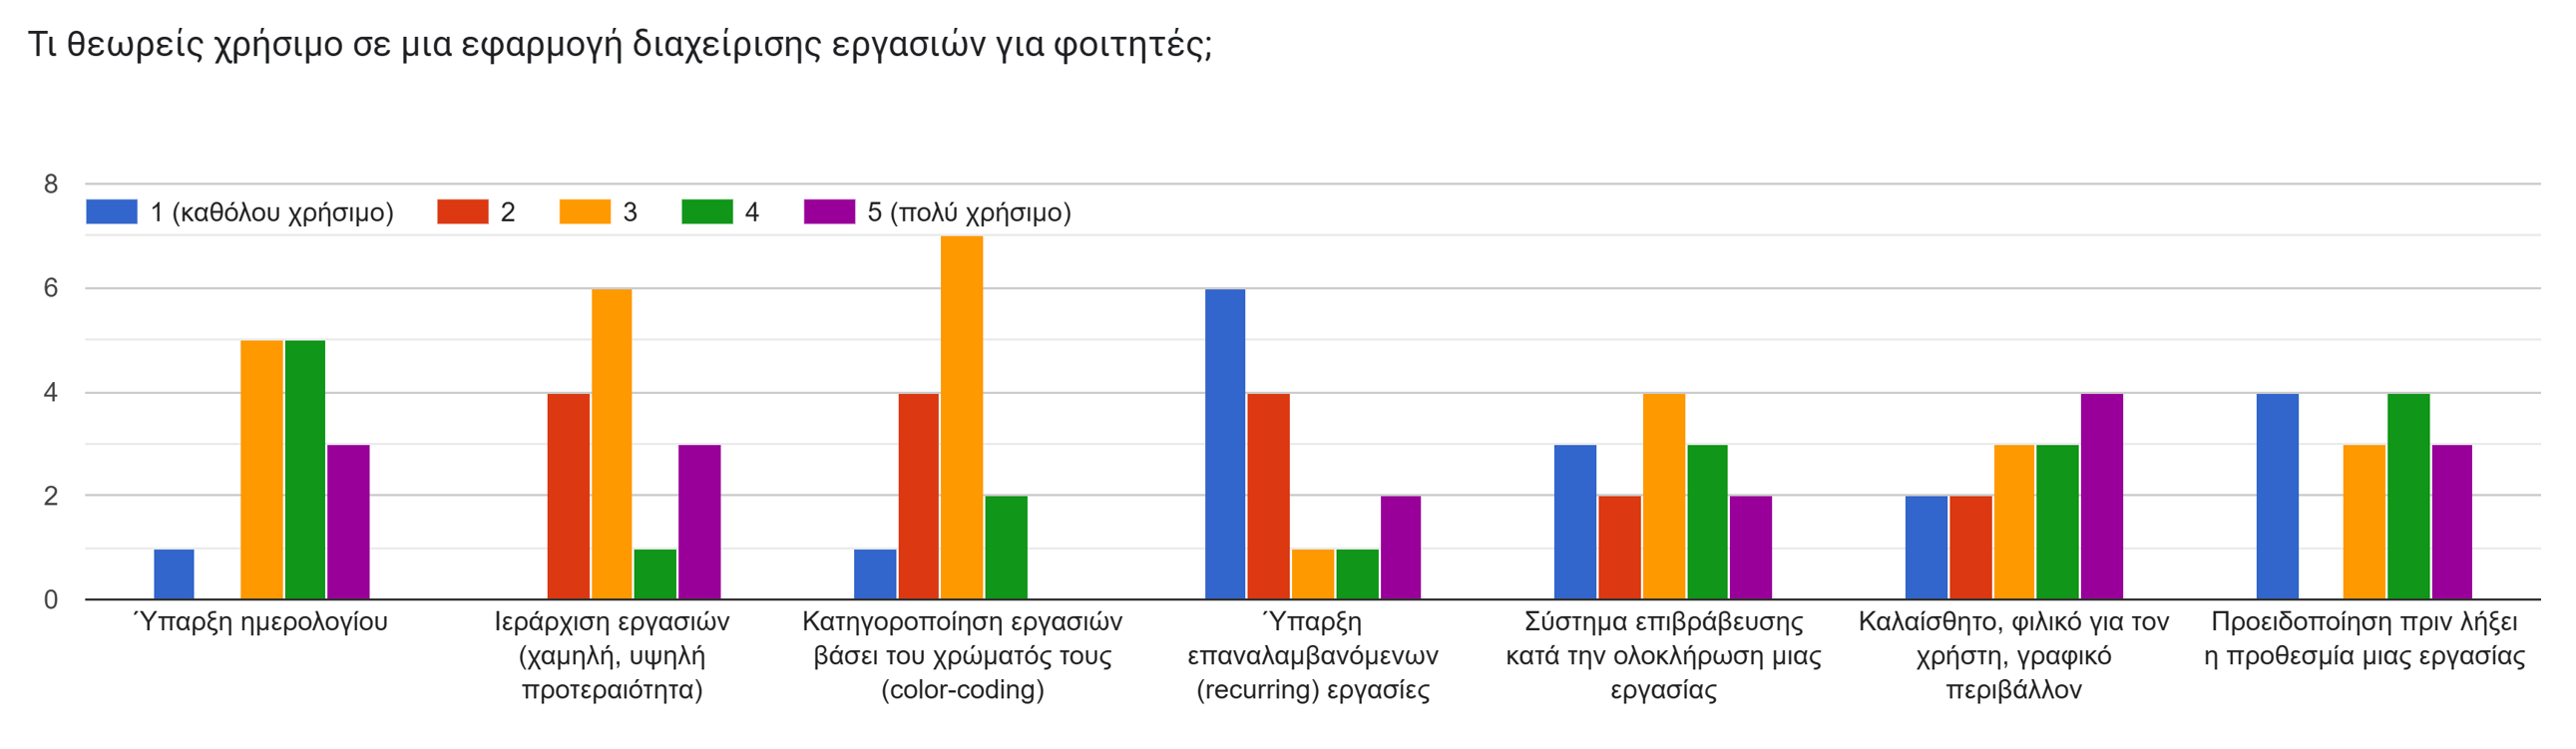
\includegraphics[width=\textwidth]{poll/poll-usefullFeatures}
                \caption{Βαθμολόγηση χαρακτηριστικών που οι φοιτητές θεωρούν χρήσιμα σε μια εφαρμογή διαχείρισης εργασιών}
                \label{fig:poll-usefullFeatures}
            \end{figure}

            Τα χαρακτηριστικά που οι φοιτητές θεωρούν χρήσιμα σε μια εφαρμογή διαχείρισης εργασιών εμφανίζονται στο \ref{fig:poll-usefullFeatures}. Παρατηρούμε πως οι φοιτητές δίνουν περισσότερο βάση στην ύπαρξη ημερολογίου, στην κατηγοριοποίηση βάση χρώματος, και στην προειδοποίηση πριν λήξει μια προθεσμία, ενώ δεν ενδιαφέρονται τόσο για την ύπαρξη επαναλαμβανόμενων εργασιών.

            Τέλος, σε κλίμακα από 1 έως 5, 6 φοιτητές βαθμολογούν με βαθμό 3 την πιθανότητα χρήσης μιας εφαρμογής διαχείρισης εργασιών σχεδιασμένη για φοιτητές, 3 φοιτητές με βαθμούς 2 και 5, και 2 φοιτητές με βαθμό 1.

        \subsection{Συμπεράσματα}
            Η έρευνα ανέδειξε ενδιαφέρουσες πτυχές σχετικά με τις δυσκολίες που αντιμετωπίζουν οι φοιτητές στη διαχείριση των εργασιών τους, καθώς και τα χαρακτηριστικά που θεωρούν ιδιαίτερα χρήσιμα σε μία εφαρμογή οργάνωσης υποχρεώσεων.

            Αρχικά, διαπιστώνεται ότι, παρά την ύπαρξη ψηφιακών εργαλείων διαχείρισης χρόνου, ένα αξιοσημείωτο ποσοστό φοιτητών εξακολουθεί να βασίζεται σε μη συστηματικές μεθόδους προγραμματισμού, όπως η απομνημόνευση των υποχρεώσεων. Επιπλέον, μεταξύ όσων χρησιμοποιούν κάποιο εργαλείο, η συντριπτική πλειοψηφία (100\%) οργανώνει υποχρεώσεις της σχολής και ένα μικρότερο ποσοστό επεκτείνει τη χρήση αυτών των εργαλείων και σε άλλους τομείς, όπως υποχρεώσεις καθημερινότητας (44,4\%), κοινωνικές δραστηριότητες (33,3\%) και προσωπική φροντίδα (33,3\%).

            Ιδιαίτερα σημαντική είναι η ανάδειξη της αναβλητικότητας (42,9\%) και της απόσπασης προσοχής από τα μέσα κοινωνικής δικτύωσης (64,3\%) ως δύο από τα πλέον συχνά προβλήματα στη διαχείριση των εργασιών. Αυτά τα ευρήματα υποδεικνύουν ότι οι φοιτητές δε χρειάζονται απλώς ένα εργαλείο καταγραφής υποχρεώσεων, αλλά μία εφαρμογή που να ενσωματώνει μηχανισμούς οι οποίοι διευκολύνουν τη συγκέντρωση και ενισχύουν τη συνέπεια στην τήρηση του προγράμματος. Η εισαγωγή ενός συστήματος επιβράβευσης, το οποίο βαθμολογείται με 3,9/5 από τους συμμετέχοντες, θα μπορούσε να λειτουργήσει ενισχυτικά στη διατήρηση κινήτρου και στη σταδιακή μείωση της αναβλητικότητας.

            Η δυσκολία τήρησης προθεσμιών αναδεικνύεται ως σημαντική πρόκληση, καθώς 78,6\% των φοιτητών έχει χάσει κάποια προθεσμία τουλάχιστον μία φορά. Επιπλέον, οι μισοί φοιτητές (50\%) έχουν τουλάχιστον μία φορά ξεχάσει ή εγκαταλείψει μία εργασία τους λόγω έλλειψης χρόνου, κούρασης ή κακής συνεργασίας ομάδας. Για να αντιμετωπιστεί αυτή η δυσκολία, η εφαρμογή θα πρέπει να ενσωματώνει υπενθυμίσεις και ειδοποιήσεις που θα προσαρμόζονται στις συνήθειες του χρήστη, επιτρέποντάς του να έχει έγκαιρη ενημέρωση σχετικά με τις προθεσμίες. Ένα σύστημα ειδοποιήσεων που θα ξεκινά με υπενθύμιση αρκετές ημέρες πριν από την προθεσμία θα μπορούσε να βελτιώσει την τήρηση των προθεσμιών.

            Όσον αφορά τα χαρακτηριστικά που θεωρούνται απαραίτητα σε μία εφαρμογή διαχείρισης εργασιών, παρατηρείται έντονο ενδιαφέρον για λειτουργίες όπως το ημερολόγιο, η ιεράρχηση εργασιών βάσει προτεραιότητας, η δυνατότητα κατηγοριοποίησης μέσω χρωμάτων και η αποστολή ειδοποιήσεων πριν από τις προθεσμίες, με όλα αυτά τα χαρακτηριστικά να λαμβάνουν μέσο όρο βαθμολογίας μεταξύ 4,2 και 4,7 σε κλίμακα 1-5. Παράλληλα, δίνεται έμφαση στη σημασία της ευχρηστίας και της αισθητικής της εφαρμογής, καθώς το φιλικό γραφικό περιβάλλον αξιολογείται με μέσο όρο 4,6/5.

            Η πρόθεση χρήσης μιας τέτοιας εφαρμογής δεν είναι απόλυτα εγγυημένη, καθώς ο μέσος όρος στην κλίμακα 1-5 φτάνει το 3,14, κάτι που δείχνει ενδιαφέρον αλλά όχι ενθουσιασμό. Αυτό υποδηλώνει ότι η αποδοχή μιας εφαρμογής εξαρτάται από το αν μπορεί να προσφέρει σημαντική βελτίωση σε σχέση με τα υπάρχοντα εργαλεία, να είναι εύκολη στη χρήση και να παρέχει σαφή οφέλη, χωρίς να προσθέτει επιπλέον γνωστικό φορτίο.

            Τα αποτελέσματα της έρευνας καταδεικνύουν ότι η ανάπτυξη μιας εφαρμογής διαχείρισης εργασιών για φοιτητές πρέπει να εστιάσει όχι μόνο στην καταγραφή υποχρεώσεων, αλλά και στη δημιουργία μηχανισμών που βοηθούν στην πειθαρχία, στη μείωση των περισπασμών και στην ενίσχυση της παραγωγικότητας. Η αποτελεσματική υλοποίηση αυτών των χαρακτηριστικών μπορεί να οδηγήσει σε μία εφαρμογή που όχι μόνο διευκολύνει τον προγραμματισμό, αλλά και βελτιώνει τη συνολική ακαδημαϊκή εμπειρία των χρηστών της.